\documentclass[1p]{elsarticle_modified}
%\bibliographystyle{elsarticle-num}

%\usepackage[colorlinks]{hyperref}
%\usepackage{abbrmath_seonhwa} %\Abb, \Ascr, \Acal ,\Abf, \Afrak
\usepackage{amsfonts}
\usepackage{amssymb}
\usepackage{amsmath}
\usepackage{amsthm}
\usepackage{scalefnt}
\usepackage{amsbsy}
\usepackage{kotex}
\usepackage{caption}
\usepackage{subfig}
\usepackage{color}
\usepackage{graphicx}
\usepackage{xcolor} %% white, black, red, green, blue, cyan, magenta, yellow
\usepackage{float}
\usepackage{setspace}
\usepackage{hyperref}

\usepackage{tikz}
\usetikzlibrary{arrows}

\usepackage{multirow}
\usepackage{array} % fixed length table
\usepackage{hhline}

%%%%%%%%%%%%%%%%%%%%%
\makeatletter
\renewcommand*\env@matrix[1][\arraystretch]{%
	\edef\arraystretch{#1}%
	\hskip -\arraycolsep
	\let\@ifnextchar\new@ifnextchar
	\array{*\c@MaxMatrixCols c}}
\makeatother %https://tex.stackexchange.com/questions/14071/how-can-i-increase-the-line-spacing-in-a-matrix
%%%%%%%%%%%%%%%

\usepackage[normalem]{ulem}

\newcommand{\msout}[1]{\ifmmode\text{\sout{\ensuremath{#1}}}\else\sout{#1}\fi}
%SOURCE: \msout is \stkout macro in https://tex.stackexchange.com/questions/20609/strikeout-in-math-mode

\newcommand{\cancel}[1]{
	\ifmmode
	{\color{red}\msout{#1}}
	\else
	{\color{red}\sout{#1}}
	\fi
}

\newcommand{\add}[1]{
	{\color{blue}\uwave{#1}}
}

\newcommand{\replace}[2]{
	\ifmmode
	{\color{red}\msout{#1}}{\color{blue}\uwave{#2}}
	\else
	{\color{red}\sout{#1}}{\color{blue}\uwave{#2}}
	\fi
}

\newcommand{\Sol}{\mathcal{S}} %segment
\newcommand{\D}{D} %diagram
\newcommand{\A}{\mathcal{A}} %arc


%%%%%%%%%%%%%%%%%%%%%%%%%%%%%5 test

\def\sl{\operatorname{\textup{SL}}(2,\Cbb)}
\def\psl{\operatorname{\textup{PSL}}(2,\Cbb)}
\def\quan{\mkern 1mu \triangleright \mkern 1mu}

\theoremstyle{definition}
\newtheorem{thm}{Theorem}[section]
\newtheorem{prop}[thm]{Proposition}
\newtheorem{lem}[thm]{Lemma}
\newtheorem{ques}[thm]{Question}
\newtheorem{cor}[thm]{Corollary}
\newtheorem{defn}[thm]{Definition}
\newtheorem{exam}[thm]{Example}
\newtheorem{rmk}[thm]{Remark}
\newtheorem{alg}[thm]{Algorithm}

\newcommand{\I}{\sqrt{-1}}
\begin{document}

%\begin{frontmatter}
%
%\title{Boundary parabolic representations of knots up to 8 crossings}
%
%%% Group authors per affiliation:
%\author{Yunhi Cho} 
%\address{Department of Mathematics, University of Seoul, Seoul, Korea}
%\ead{yhcho@uos.ac.kr}
%
%
%\author{Seonhwa Kim} %\fnref{s_kim}}
%\address{Center for Geometry and Physics, Institute for Basic Science, Pohang, 37673, Korea}
%\ead{ryeona17@ibs.re.kr}
%
%\author{Hyuk Kim}
%\address{Department of Mathematical Sciences, Seoul National University, Seoul 08826, Korea}
%\ead{hyukkim@snu.ac.kr}
%
%\author{Seokbeom Yoon}
%\address{Department of Mathematical Sciences, Seoul National University, Seoul, 08826,  Korea}
%\ead{sbyoon15@snu.ac.kr}
%
%\begin{abstract}
%We find all boundary parabolic representation of knots up to 8 crossings.
%
%\end{abstract}
%\begin{keyword}
%    \MSC[2010] 57M25 
%\end{keyword}
%
%\end{frontmatter}

%\linenumbers
%\tableofcontents
%
\newcommand\colored[1]{\textcolor{white}{\rule[-0.35ex]{0.8em}{1.4ex}}\kern-0.8em\color{red} #1}%
%\newcommand\colored[1]{\textcolor{white}{ #1}\kern-2.17ex	\textcolor{white}{ #1}\kern-1.81ex	\textcolor{white}{ #1}\kern-2.15ex\color{red}#1	}

{\Large $\underline{12a_{0547}~(K12a_{0547})}$}

\setlength{\tabcolsep}{10pt}
\renewcommand{\arraystretch}{1.6}
\vspace{1cm}\begin{tabular}{m{100pt}>{\centering\arraybackslash}m{274pt}}
\multirow{5}{120pt}{
	\centering
	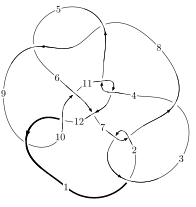
\includegraphics[width=112pt]{../../../GIT/diagram.site/Diagrams/png/1348_12a_0547.png}\\
\ \ \ A knot diagram\footnotemark}&
\allowdisplaybreaks
\textbf{Linearized knot diagam} \\
\cline{2-2}
 &
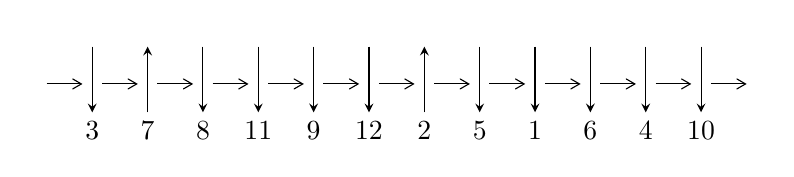
\begin{tikzpicture}[x=20pt, y=17pt]
	% nodes
	\node (C0) at (0, 0) {};
	\node (C1) at (1, 0) {};
	\node (C1U) at (1, +1) {};
	\node (C1D) at (1, -1) {3};

	\node (C2) at (2, 0) {};
	\node (C2U) at (2, +1) {};
	\node (C2D) at (2, -1) {7};

	\node (C3) at (3, 0) {};
	\node (C3U) at (3, +1) {};
	\node (C3D) at (3, -1) {8};

	\node (C4) at (4, 0) {};
	\node (C4U) at (4, +1) {};
	\node (C4D) at (4, -1) {11};

	\node (C5) at (5, 0) {};
	\node (C5U) at (5, +1) {};
	\node (C5D) at (5, -1) {9};

	\node (C6) at (6, 0) {};
	\node (C6U) at (6, +1) {};
	\node (C6D) at (6, -1) {12};

	\node (C7) at (7, 0) {};
	\node (C7U) at (7, +1) {};
	\node (C7D) at (7, -1) {2};

	\node (C8) at (8, 0) {};
	\node (C8U) at (8, +1) {};
	\node (C8D) at (8, -1) {5};

	\node (C9) at (9, 0) {};
	\node (C9U) at (9, +1) {};
	\node (C9D) at (9, -1) {1};

	\node (C10) at (10, 0) {};
	\node (C10U) at (10, +1) {};
	\node (C10D) at (10, -1) {6};

	\node (C11) at (11, 0) {};
	\node (C11U) at (11, +1) {};
	\node (C11D) at (11, -1) {4};

	\node (C12) at (12, 0) {};
	\node (C12U) at (12, +1) {};
	\node (C12D) at (12, -1) {10};
	\node (C13) at (13, 0) {};

	% arrows
	\draw[->,>={angle 60}]
	(C0) edge (C1) (C1) edge (C2) (C2) edge (C3) (C3) edge (C4) (C4) edge (C5) (C5) edge (C6) (C6) edge (C7) (C7) edge (C8) (C8) edge (C9) (C9) edge (C10) (C10) edge (C11) (C11) edge (C12) (C12) edge (C13) ;	\draw[->,>=stealth]
	(C1U) edge (C1D) (C2D) edge (C2U) (C3U) edge (C3D) (C4U) edge (C4D) (C5U) edge (C5D) (C6U) edge (C6D) (C7D) edge (C7U) (C8U) edge (C8D) (C9U) edge (C9D) (C10U) edge (C10D) (C11U) edge (C11D) (C12U) edge (C12D) ;
	\end{tikzpicture} \\
\hhline{~~} \\& 
\textbf{Solving Sequence} \\ \cline{2-2} 
 &
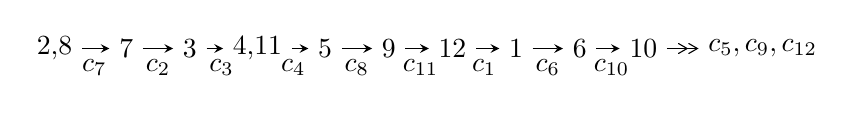
\begin{tikzpicture}[x=23pt, y=7pt]
	% node
	\node (A0) at (-1/8, 0) {2,8};
	\node (A1) at (1, 0) {7};
	\node (A2) at (2, 0) {3};
	\node (A3) at (49/16, 0) {4,11};
	\node (A4) at (33/8, 0) {5};
	\node (A5) at (41/8, 0) {9};
	\node (A6) at (49/8, 0) {12};
	\node (A7) at (57/8, 0) {1};
	\node (A8) at (65/8, 0) {6};
	\node (A9) at (73/8, 0) {10};
	\node (C1) at (1/2, -1) {$c_{7}$};
	\node (C2) at (3/2, -1) {$c_{2}$};
	\node (C3) at (5/2, -1) {$c_{3}$};
	\node (C4) at (29/8, -1) {$c_{4}$};
	\node (C5) at (37/8, -1) {$c_{8}$};
	\node (C6) at (45/8, -1) {$c_{11}$};
	\node (C7) at (53/8, -1) {$c_{1}$};
	\node (C8) at (61/8, -1) {$c_{6}$};
	\node (C9) at (69/8, -1) {$c_{10}$};
	\node (A10) at (11, 0) {$c_{5},c_{9},c_{12}$};

	% edge
	\draw[->,>=stealth]	
	(A0) edge (A1) (A1) edge (A2) (A2) edge (A3) (A3) edge (A4) (A4) edge (A5) (A5) edge (A6) (A6) edge (A7) (A7) edge (A8) (A8) edge (A9) ;
	\draw[->>,>={angle 60}]	
	(A9) edge (A10);
\end{tikzpicture} \\ 

\end{tabular} \\

\footnotetext{
The image of knot diagram is generated by the software ``\textbf{Draw programme}" developed by Andrew Bartholomew(\url{http://www.layer8.co.uk/maths/draw/index.htm\#Running-draw}), where we modified some parts for our purpose(\url{https://github.com/CATsTAILs/LinksPainter}).
}\phantom \\ \newline 
\centering \textbf{Ideals for irreducible components\footnotemark of $X_{\text{par}}$} 
 
\begin{align*}
I^u_{1}&=\langle 
-1.82820\times10^{271} u^{152}+1.44234\times10^{271} u^{151}+\cdots+2.04979\times10^{271} b+3.56914\times10^{272},\\
\phantom{I^u_{1}}&\phantom{= \langle  }4.13842\times10^{272} u^{152}+4.80709\times10^{272} u^{151}+\cdots+2.25477\times10^{272} a+5.49438\times10^{273},\\
\phantom{I^u_{1}}&\phantom{= \langle  }u^{153}+u^{152}+\cdots+28 u+11\rangle \\
I^u_{2}&=\langle 
-15 u^{36}+4 u^{35}+\cdots+b+12,\;3 u^{36}- u^{35}+\cdots+a+4,\;u^{37}+10 u^{35}+\cdots+7 u^2+1\rangle \\
\\
\end{align*}
\raggedright * 2 irreducible components of $\dim_{\mathbb{C}}=0$, with total 190 representations.\\
\footnotetext{All coefficients of polynomials are rational numbers. But the coefficients are sometimes approximated in decimal forms when there is not enough margin.}
\newpage
\renewcommand{\arraystretch}{1}
\centering \section*{I. $I^u_{1}= \langle -1.83\times10^{271} u^{152}+1.44\times10^{271} u^{151}+\cdots+2.05\times10^{271} b+3.57\times10^{272},\;4.14\times10^{272} u^{152}+4.81\times10^{272} u^{151}+\cdots+2.25\times10^{272} a+5.49\times10^{273},\;u^{153}+u^{152}+\cdots+28 u+11 \rangle$}
\flushleft \textbf{(i) Arc colorings}\\
\begin{tabular}{m{7pt} m{180pt} m{7pt} m{180pt} }
\flushright $a_{2}=$&$\begin{pmatrix}0\\u\end{pmatrix}$ \\
\flushright $a_{8}=$&$\begin{pmatrix}1\\0\end{pmatrix}$ \\
\flushright $a_{7}=$&$\begin{pmatrix}1\\u^2\end{pmatrix}$ \\
\flushright $a_{3}=$&$\begin{pmatrix}u\\u^3+u\end{pmatrix}$ \\
\flushright $a_{4}=$&$\begin{pmatrix}- u^3\\u^3+u\end{pmatrix}$ \\
\flushright $a_{11}=$&$\begin{pmatrix}-1.83540 u^{152}-2.13196 u^{151}+\cdots-55.6512 u-24.3678\\0.891895 u^{152}-0.703650 u^{151}+\cdots-15.7291 u-17.4122\end{pmatrix}$ \\
\flushright $a_{5}=$&$\begin{pmatrix}-3.07699 u^{152}+0.677463 u^{151}+\cdots-31.4818 u-0.617562\\-0.627358 u^{152}-1.90774 u^{151}+\cdots-44.2921 u-19.0364\end{pmatrix}$ \\
\flushright $a_{9}=$&$\begin{pmatrix}0.541198 u^{152}-4.00467 u^{151}+\cdots-73.7467 u-47.3026\\1.32157 u^{152}+0.752987 u^{151}+\cdots+18.8733 u-1.48239\end{pmatrix}$ \\
\flushright $a_{12}=$&$\begin{pmatrix}-2.06938 u^{152}-1.82937 u^{151}+\cdots-53.0326 u-22.5137\\0.934884 u^{152}-1.02868 u^{151}+\cdots-17.9375 u-17.6217\end{pmatrix}$ \\
\flushright $a_{1}=$&$\begin{pmatrix}u^3\\u^5+u^3+u\end{pmatrix}$ \\
\flushright $a_{6}=$&$\begin{pmatrix}-2.75509 u^{152}+0.779317 u^{151}+\cdots-25.6683 u-2.59189\\-1.43719 u^{152}-3.10153 u^{151}+\cdots-82.2229 u-39.1923\end{pmatrix}$ \\
\flushright $a_{10}=$&$\begin{pmatrix}-1.72401 u^{152}-2.92931 u^{151}+\cdots-75.4883 u-35.5372\\1.63954 u^{152}-0.541052 u^{151}+\cdots+7.50025 u-9.41830\end{pmatrix}$\\&\end{tabular}
\flushleft \textbf{(ii) Obstruction class $= -1$}\\~\\
\flushleft \textbf{(iii) Cusp Shapes $= 4.17995 u^{152}-1.07008 u^{151}+\cdots+20.1517 u-47.8921$}\\~\\
\newpage\renewcommand{\arraystretch}{1}
\flushleft \textbf{(iv) u-Polynomials at the component}\newline \\
\begin{tabular}{m{50pt}|m{274pt}}
Crossings & \hspace{64pt}u-Polynomials at each crossing \\
\hline $$\begin{aligned}c_{1}\end{aligned}$$&$\begin{aligned}
&u^{153}+77 u^{152}+\cdots-1548 u-121
\end{aligned}$\\
\hline $$\begin{aligned}c_{2},c_{7}\end{aligned}$$&$\begin{aligned}
&u^{153}+u^{152}+\cdots+28 u+11
\end{aligned}$\\
\hline $$\begin{aligned}c_{3}\end{aligned}$$&$\begin{aligned}
&u^{153}- u^{152}+\cdots+13334880 u+1770791
\end{aligned}$\\
\hline $$\begin{aligned}c_{4},c_{11}\end{aligned}$$&$\begin{aligned}
&u^{153}+2 u^{152}+\cdots+3 u+1
\end{aligned}$\\
\hline $$\begin{aligned}c_{5},c_{8}\end{aligned}$$&$\begin{aligned}
&u^{153}-50 u^{151}+\cdots+8395 u+10331
\end{aligned}$\\
\hline $$\begin{aligned}c_{6}\end{aligned}$$&$\begin{aligned}
&u^{153}+u^{152}+\cdots+869544 u+253007
\end{aligned}$\\
\hline $$\begin{aligned}c_{9},c_{12}\end{aligned}$$&$\begin{aligned}
&u^{153}-4 u^{152}+\cdots-52195 u+4961
\end{aligned}$\\
\hline $$\begin{aligned}c_{10}\end{aligned}$$&$\begin{aligned}
&u^{153}- u^{152}+\cdots+35046 u+9439
\end{aligned}$\\
\hline
\end{tabular}\\~\\
\newpage\renewcommand{\arraystretch}{1}
\flushleft \textbf{(v) Riley Polynomials at the component}\newline \\
\begin{tabular}{m{50pt}|m{274pt}}
Crossings & \hspace{64pt}Riley Polynomials at each crossing \\
\hline $$\begin{aligned}c_{1}\end{aligned}$$&$\begin{aligned}
&y^{153}+5 y^{152}+\cdots-286508 y-14641
\end{aligned}$\\
\hline $$\begin{aligned}c_{2},c_{7}\end{aligned}$$&$\begin{aligned}
&y^{153}+77 y^{152}+\cdots-1548 y-121
\end{aligned}$\\
\hline $$\begin{aligned}c_{3}\end{aligned}$$&$\begin{aligned}
&y^{153}-67 y^{152}+\cdots-141584742282518 y-3135700765681
\end{aligned}$\\
\hline $$\begin{aligned}c_{4},c_{11}\end{aligned}$$&$\begin{aligned}
&y^{153}+84 y^{152}+\cdots-39 y-1
\end{aligned}$\\
\hline $$\begin{aligned}c_{5},c_{8}\end{aligned}$$&$\begin{aligned}
&y^{153}-100 y^{152}+\cdots+4473444915 y-106729561
\end{aligned}$\\
\hline $$\begin{aligned}c_{6}\end{aligned}$$&$\begin{aligned}
&y^{153}+25 y^{152}+\cdots-1962648262454 y-64012542049
\end{aligned}$\\
\hline $$\begin{aligned}c_{9},c_{12}\end{aligned}$$&$\begin{aligned}
&y^{153}+80 y^{152}+\cdots-798994097 y-24611521
\end{aligned}$\\
\hline $$\begin{aligned}c_{10}\end{aligned}$$&$\begin{aligned}
&y^{153}+17 y^{152}+\cdots-7057634132 y-89094721
\end{aligned}$\\
\hline
\end{tabular}\\~\\
\newpage\flushleft \textbf{(vi) Complex Volumes and Cusp Shapes}
$$\begin{array}{c|c|c}  
\text{Solutions to }I^u_{1}& \I (\text{vol} + \sqrt{-1}CS) & \text{Cusp shape}\\
 \hline 
\begin{aligned}
u &= -0.803169 + 0.577760 I \\
a &= \phantom{-}0.654727 - 0.658081 I \\
b &= -2.16547 + 0.07601 I\end{aligned}
 & \phantom{-}2.89636 + 2.62923 I & \phantom{-0.000000 } 0 \\ \hline\begin{aligned}
u &= -0.803169 - 0.577760 I \\
a &= \phantom{-}0.654727 + 0.658081 I \\
b &= -2.16547 - 0.07601 I\end{aligned}
 & \phantom{-}2.89636 - 2.62923 I & \phantom{-0.000000 } 0 \\ \hline\begin{aligned}
u &= -1.004370 + 0.112798 I \\
a &= -0.307076 - 0.833264 I \\
b &= \phantom{-}0.592813 + 1.118070 I\end{aligned}
 & -1.59495 + 1.22097 I & \phantom{-0.000000 } 0 \\ \hline\begin{aligned}
u &= -1.004370 - 0.112798 I \\
a &= -0.307076 + 0.833264 I \\
b &= \phantom{-}0.592813 - 1.118070 I\end{aligned}
 & -1.59495 - 1.22097 I & \phantom{-0.000000 } 0 \\ \hline\begin{aligned}
u &= -0.420378 + 0.885705 I \\
a &= \phantom{-}1.45676 + 0.24596 I \\
b &= -1.23957 - 0.84798 I\end{aligned}
 & \phantom{-}1.16632 + 2.69264 I & \phantom{-0.000000 } 0 \\ \hline\begin{aligned}
u &= -0.420378 - 0.885705 I \\
a &= \phantom{-}1.45676 - 0.24596 I \\
b &= -1.23957 + 0.84798 I\end{aligned}
 & \phantom{-}1.16632 - 2.69264 I & \phantom{-0.000000 } 0 \\ \hline\begin{aligned}
u &= -0.169016 + 1.013590 I \\
a &= \phantom{-}1.214710 + 0.245532 I \\
b &= -0.462782 - 0.735315 I\end{aligned}
 & -1.48405 + 1.57407 I & \phantom{-0.000000 } 0 \\ \hline\begin{aligned}
u &= -0.169016 - 1.013590 I \\
a &= \phantom{-}1.214710 - 0.245532 I \\
b &= -0.462782 + 0.735315 I\end{aligned}
 & -1.48405 - 1.57407 I & \phantom{-0.000000 } 0 \\ \hline\begin{aligned}
u &= \phantom{-}0.661362 + 0.709297 I \\
a &= \phantom{-}0.463802 - 0.665196 I \\
b &= \phantom{-}1.51391 + 0.38433 I\end{aligned}
 & \phantom{-}1.30435 + 5.87704 I & \phantom{-0.000000 } 0 \\ \hline\begin{aligned}
u &= \phantom{-}0.661362 - 0.709297 I \\
a &= \phantom{-}0.463802 + 0.665196 I \\
b &= \phantom{-}1.51391 - 0.38433 I\end{aligned}
 & \phantom{-}1.30435 - 5.87704 I & \phantom{-0.000000 } 0\\
 \hline 
 \end{array}$$\newpage$$\begin{array}{c|c|c}  
\text{Solutions to }I^u_{1}& \I (\text{vol} + \sqrt{-1}CS) & \text{Cusp shape}\\
 \hline 
\begin{aligned}
u &= -0.661394 + 0.698725 I \\
a &= -0.054834 + 0.347458 I \\
b &= \phantom{-}1.60907 + 0.63444 I\end{aligned}
 & \phantom{-}7.98668 - 5.17937 I & \phantom{-0.000000 } 0 \\ \hline\begin{aligned}
u &= -0.661394 - 0.698725 I \\
a &= -0.054834 - 0.347458 I \\
b &= \phantom{-}1.60907 - 0.63444 I\end{aligned}
 & \phantom{-}7.98668 + 5.17937 I & \phantom{-0.000000 } 0 \\ \hline\begin{aligned}
u &= \phantom{-}0.926965 + 0.468778 I \\
a &= -0.899004 + 0.412334 I \\
b &= \phantom{-}2.08791 - 1.45289 I\end{aligned}
 & \phantom{-}0.49601 - 3.67330 I & \phantom{-0.000000 } 0 \\ \hline\begin{aligned}
u &= \phantom{-}0.926965 - 0.468778 I \\
a &= -0.899004 - 0.412334 I \\
b &= \phantom{-}2.08791 + 1.45289 I\end{aligned}
 & \phantom{-}0.49601 + 3.67330 I & \phantom{-0.000000 } 0 \\ \hline\begin{aligned}
u &= \phantom{-}0.922348 + 0.250824 I \\
a &= \phantom{-}0.432284 - 1.050650 I \\
b &= -1.42601 + 1.70545 I\end{aligned}
 & \phantom{-}0.69176 - 1.30939 I & \phantom{-0.000000 } 0 \\ \hline\begin{aligned}
u &= \phantom{-}0.922348 - 0.250824 I \\
a &= \phantom{-}0.432284 + 1.050650 I \\
b &= -1.42601 - 1.70545 I\end{aligned}
 & \phantom{-}0.69176 + 1.30939 I & \phantom{-0.000000 } 0 \\ \hline\begin{aligned}
u &= \phantom{-}0.599653 + 0.866993 I \\
a &= -0.12882 - 1.44661 I \\
b &= \phantom{-}1.282060 - 0.139973 I\end{aligned}
 & \phantom{-}0.836296 - 0.978230 I & \phantom{-0.000000 } 0 \\ \hline\begin{aligned}
u &= \phantom{-}0.599653 - 0.866993 I \\
a &= -0.12882 + 1.44661 I \\
b &= \phantom{-}1.282060 + 0.139973 I\end{aligned}
 & \phantom{-}0.836296 + 0.978230 I & \phantom{-0.000000 } 0 \\ \hline\begin{aligned}
u &= \phantom{-}0.024048 + 1.060330 I \\
a &= \phantom{-}1.70255 + 0.01296 I \\
b &= -0.953502 - 0.444769 I\end{aligned}
 & \phantom{-}0.19382 + 2.04626 I & \phantom{-0.000000 } 0 \\ \hline\begin{aligned}
u &= \phantom{-}0.024048 - 1.060330 I \\
a &= \phantom{-}1.70255 - 0.01296 I \\
b &= -0.953502 + 0.444769 I\end{aligned}
 & \phantom{-}0.19382 - 2.04626 I & \phantom{-0.000000 } 0\\
 \hline 
 \end{array}$$\newpage$$\begin{array}{c|c|c}  
\text{Solutions to }I^u_{1}& \I (\text{vol} + \sqrt{-1}CS) & \text{Cusp shape}\\
 \hline 
\begin{aligned}
u &= -0.885318 + 0.300352 I \\
a &= \phantom{-}0.282592 + 0.613095 I \\
b &= -1.86384 - 1.14675 I\end{aligned}
 & \phantom{-}2.3619 + 14.1579 I & \phantom{-0.000000 } 0 \\ \hline\begin{aligned}
u &= -0.885318 - 0.300352 I \\
a &= \phantom{-}0.282592 - 0.613095 I \\
b &= -1.86384 + 1.14675 I\end{aligned}
 & \phantom{-}2.3619 - 14.1579 I & \phantom{-0.000000 } 0 \\ \hline\begin{aligned}
u &= -0.538737 + 0.761034 I \\
a &= -0.809151 - 1.144800 I \\
b &= -1.272290 + 0.084596 I\end{aligned}
 & \phantom{-}4.31832 - 2.17917 I & \phantom{-0.000000 } 0 \\ \hline\begin{aligned}
u &= -0.538737 - 0.761034 I \\
a &= -0.809151 + 1.144800 I \\
b &= -1.272290 - 0.084596 I\end{aligned}
 & \phantom{-}4.31832 + 2.17917 I & \phantom{-0.000000 } 0 \\ \hline\begin{aligned}
u &= \phantom{-}0.265107 + 1.037410 I \\
a &= -0.391450 - 0.151234 I \\
b &= \phantom{-}0.808245 + 0.272149 I\end{aligned}
 & \phantom{-}1.63828 + 3.80010 I & \phantom{-0.000000 } 0 \\ \hline\begin{aligned}
u &= \phantom{-}0.265107 - 1.037410 I \\
a &= -0.391450 + 0.151234 I \\
b &= \phantom{-}0.808245 - 0.272149 I\end{aligned}
 & \phantom{-}1.63828 - 3.80010 I & \phantom{-0.000000 } 0 \\ \hline\begin{aligned}
u &= -0.529733 + 0.745288 I \\
a &= \phantom{-}0.27196 - 1.60407 I \\
b &= -0.847186 + 0.569319 I\end{aligned}
 & \phantom{-}1.48585 - 6.62716 I & \phantom{-0.000000 } 0 \\ \hline\begin{aligned}
u &= -0.529733 - 0.745288 I \\
a &= \phantom{-}0.27196 + 1.60407 I \\
b &= -0.847186 - 0.569319 I\end{aligned}
 & \phantom{-}1.48585 + 6.62716 I & \phantom{-0.000000 } 0 \\ \hline\begin{aligned}
u &= -0.626068 + 0.894564 I \\
a &= \phantom{-}0.64894 + 2.15812 I \\
b &= \phantom{-}1.34997 - 1.01960 I\end{aligned}
 & \phantom{-}7.41917 + 0.20736 I & \phantom{-0.000000 } 0 \\ \hline\begin{aligned}
u &= -0.626068 - 0.894564 I \\
a &= \phantom{-}0.64894 - 2.15812 I \\
b &= \phantom{-}1.34997 + 1.01960 I\end{aligned}
 & \phantom{-}7.41917 - 0.20736 I & \phantom{-0.000000 } 0\\
 \hline 
 \end{array}$$\newpage$$\begin{array}{c|c|c}  
\text{Solutions to }I^u_{1}& \I (\text{vol} + \sqrt{-1}CS) & \text{Cusp shape}\\
 \hline 
\begin{aligned}
u &= \phantom{-}0.113240 + 1.098040 I \\
a &= -2.40907 + 1.47465 I \\
b &= \phantom{-}1.004810 - 0.952987 I\end{aligned}
 & -5.34213 - 1.63294 I & \phantom{-0.000000 } 0 \\ \hline\begin{aligned}
u &= \phantom{-}0.113240 - 1.098040 I \\
a &= -2.40907 - 1.47465 I \\
b &= \phantom{-}1.004810 + 0.952987 I\end{aligned}
 & -5.34213 + 1.63294 I & \phantom{-0.000000 } 0 \\ \hline\begin{aligned}
u &= \phantom{-}0.737210 + 0.499189 I \\
a &= \phantom{-}0.035993 - 0.473925 I \\
b &= -1.232050 + 0.370722 I\end{aligned}
 & \phantom{-}5.42547 + 0.75189 I & \phantom{-0.000000 } 0 \\ \hline\begin{aligned}
u &= \phantom{-}0.737210 - 0.499189 I \\
a &= \phantom{-}0.035993 + 0.473925 I \\
b &= -1.232050 - 0.370722 I\end{aligned}
 & \phantom{-}5.42547 - 0.75189 I & \phantom{-0.000000 } 0 \\ \hline\begin{aligned}
u &= -0.427201 + 1.025550 I \\
a &= \phantom{-}1.46652 - 2.59746 I \\
b &= -2.03822 - 0.26994 I\end{aligned}
 & -0.07991 + 1.48262 I & \phantom{-0.000000 } 0 \\ \hline\begin{aligned}
u &= -0.427201 - 1.025550 I \\
a &= \phantom{-}1.46652 + 2.59746 I \\
b &= -2.03822 + 0.26994 I\end{aligned}
 & -0.07991 - 1.48262 I & \phantom{-0.000000 } 0 \\ \hline\begin{aligned}
u &= \phantom{-}0.524046 + 0.983672 I \\
a &= -0.204309 + 0.610614 I \\
b &= \phantom{-}0.244671 - 0.234525 I\end{aligned}
 & \phantom{-}2.01558 + 2.87049 I & \phantom{-0.000000 } 0 \\ \hline\begin{aligned}
u &= \phantom{-}0.524046 - 0.983672 I \\
a &= -0.204309 - 0.610614 I \\
b &= \phantom{-}0.244671 + 0.234525 I\end{aligned}
 & \phantom{-}2.01558 - 2.87049 I & \phantom{-0.000000 } 0 \\ \hline\begin{aligned}
u &= \phantom{-}0.795132 + 0.784678 I \\
a &= \phantom{-}0.418719 + 1.070430 I \\
b &= -2.11529 - 0.37904 I\end{aligned}
 & \phantom{-}5.30275 + 10.77780 I & \phantom{-0.000000 } 0 \\ \hline\begin{aligned}
u &= \phantom{-}0.795132 - 0.784678 I \\
a &= \phantom{-}0.418719 - 1.070430 I \\
b &= -2.11529 + 0.37904 I\end{aligned}
 & \phantom{-}5.30275 - 10.77780 I & \phantom{-0.000000 } 0\\
 \hline 
 \end{array}$$\newpage$$\begin{array}{c|c|c}  
\text{Solutions to }I^u_{1}& \I (\text{vol} + \sqrt{-1}CS) & \text{Cusp shape}\\
 \hline 
\begin{aligned}
u &= -0.467919 + 1.030120 I \\
a &= -0.486150 + 0.390238 I \\
b &= \phantom{-}1.266510 + 0.358123 I\end{aligned}
 & -4.17331 - 3.13943 I & \phantom{-0.000000 } 0 \\ \hline\begin{aligned}
u &= -0.467919 - 1.030120 I \\
a &= -0.486150 - 0.390238 I \\
b &= \phantom{-}1.266510 - 0.358123 I\end{aligned}
 & -4.17331 + 3.13943 I & \phantom{-0.000000 } 0 \\ \hline\begin{aligned}
u &= -0.422936 + 1.051470 I \\
a &= -1.64652 - 2.71399 I \\
b &= -0.279492 + 1.009320 I\end{aligned}
 & \phantom{-}2.80395 - 0.18184 I & \phantom{-0.000000 } 0 \\ \hline\begin{aligned}
u &= -0.422936 - 1.051470 I \\
a &= -1.64652 + 2.71399 I \\
b &= -0.279492 - 1.009320 I\end{aligned}
 & \phantom{-}2.80395 + 0.18184 I & \phantom{-0.000000 } 0 \\ \hline\begin{aligned}
u &= -0.728290 + 0.455821 I \\
a &= -0.255788 - 0.431460 I \\
b &= -1.71113 - 0.25408 I\end{aligned}
 & \phantom{-}5.24838 + 3.35209 I & \phantom{-0.000000 } 0 \\ \hline\begin{aligned}
u &= -0.728290 - 0.455821 I \\
a &= -0.255788 + 0.431460 I \\
b &= -1.71113 + 0.25408 I\end{aligned}
 & \phantom{-}5.24838 - 3.35209 I & \phantom{-0.000000 } 0 \\ \hline\begin{aligned}
u &= -0.805772 + 0.293840 I \\
a &= \phantom{-}0.125125 - 0.537652 I \\
b &= \phantom{-}1.59272 + 0.94279 I\end{aligned}
 & -0.88656 + 8.08747 I & \phantom{-0.000000 } 0 \\ \hline\begin{aligned}
u &= -0.805772 - 0.293840 I \\
a &= \phantom{-}0.125125 + 0.537652 I \\
b &= \phantom{-}1.59272 - 0.94279 I\end{aligned}
 & -0.88656 - 8.08747 I & \phantom{-0.000000 } 0 \\ \hline\begin{aligned}
u &= -0.415484 + 1.068520 I \\
a &= -1.264150 + 0.217576 I \\
b &= \phantom{-}1.020550 + 0.631809 I\end{aligned}
 & -3.51137 - 3.38573 I & \phantom{-0.000000 } 0 \\ \hline\begin{aligned}
u &= -0.415484 - 1.068520 I \\
a &= -1.264150 - 0.217576 I \\
b &= \phantom{-}1.020550 - 0.631809 I\end{aligned}
 & -3.51137 + 3.38573 I & \phantom{-0.000000 } 0\\
 \hline 
 \end{array}$$\newpage$$\begin{array}{c|c|c}  
\text{Solutions to }I^u_{1}& \I (\text{vol} + \sqrt{-1}CS) & \text{Cusp shape}\\
 \hline 
\begin{aligned}
u &= \phantom{-}0.436413 + 1.062230 I \\
a &= -2.81312 + 1.71557 I \\
b &= \phantom{-}1.01179 - 1.77752 I\end{aligned}
 & -3.07142 + 1.23078 I & \phantom{-0.000000 } 0 \\ \hline\begin{aligned}
u &= \phantom{-}0.436413 - 1.062230 I \\
a &= -2.81312 - 1.71557 I \\
b &= \phantom{-}1.01179 + 1.77752 I\end{aligned}
 & -3.07142 - 1.23078 I & \phantom{-0.000000 } 0 \\ \hline\begin{aligned}
u &= \phantom{-}0.214188 + 0.812689 I \\
a &= \phantom{-}0.522372 + 0.212518 I \\
b &= -0.129247 - 0.290374 I\end{aligned}
 & -0.573771 + 1.117010 I & \phantom{-0.000000 } 0 \\ \hline\begin{aligned}
u &= \phantom{-}0.214188 - 0.812689 I \\
a &= \phantom{-}0.522372 - 0.212518 I \\
b &= -0.129247 + 0.290374 I\end{aligned}
 & -0.573771 - 1.117010 I & \phantom{-0.000000 } 0 \\ \hline\begin{aligned}
u &= \phantom{-}0.791592 + 0.279934 I \\
a &= \phantom{-}0.010624 + 0.208496 I \\
b &= \phantom{-}1.83748 - 0.03341 I\end{aligned}
 & \phantom{-}5.85581 - 7.23825 I & \phantom{-0.000000 } 0 \\ \hline\begin{aligned}
u &= \phantom{-}0.791592 - 0.279934 I \\
a &= \phantom{-}0.010624 - 0.208496 I \\
b &= \phantom{-}1.83748 + 0.03341 I\end{aligned}
 & \phantom{-}5.85581 + 7.23825 I & \phantom{-0.000000 } 0 \\ \hline\begin{aligned}
u &= \phantom{-}0.484218 + 1.074660 I \\
a &= \phantom{-}0.80584 - 3.69106 I \\
b &= \phantom{-}1.57664 + 1.61174 I\end{aligned}
 & -2.70678 + 5.64464 I & \phantom{-0.000000 } 0 \\ \hline\begin{aligned}
u &= \phantom{-}0.484218 - 1.074660 I \\
a &= \phantom{-}0.80584 + 3.69106 I \\
b &= \phantom{-}1.57664 - 1.61174 I\end{aligned}
 & -2.70678 - 5.64464 I & \phantom{-0.000000 } 0 \\ \hline\begin{aligned}
u &= \phantom{-}0.355257 + 1.125980 I \\
a &= -1.022580 + 0.111630 I \\
b &= \phantom{-}0.030616 + 0.297694 I\end{aligned}
 & -7.39263 + 2.02832 I & \phantom{-0.000000 } 0 \\ \hline\begin{aligned}
u &= \phantom{-}0.355257 - 1.125980 I \\
a &= -1.022580 - 0.111630 I \\
b &= \phantom{-}0.030616 - 0.297694 I\end{aligned}
 & -7.39263 - 2.02832 I & \phantom{-0.000000 } 0\\
 \hline 
 \end{array}$$\newpage$$\begin{array}{c|c|c}  
\text{Solutions to }I^u_{1}& \I (\text{vol} + \sqrt{-1}CS) & \text{Cusp shape}\\
 \hline 
\begin{aligned}
u &= -0.495307 + 1.075110 I \\
a &= \phantom{-}1.37526 + 2.72517 I \\
b &= \phantom{-}0.313367 - 1.252430 I\end{aligned}
 & \phantom{-}3.36604 - 6.63400 I & \phantom{-0.000000 } 0 \\ \hline\begin{aligned}
u &= -0.495307 - 1.075110 I \\
a &= \phantom{-}1.37526 - 2.72517 I \\
b &= \phantom{-}0.313367 + 1.252430 I\end{aligned}
 & \phantom{-}3.36604 + 6.63400 I & \phantom{-0.000000 } 0 \\ \hline\begin{aligned}
u &= -0.498143 + 1.073910 I \\
a &= -1.19365 + 1.96600 I \\
b &= \phantom{-}1.73648 - 0.00647 I\end{aligned}
 & -2.99168 - 3.47198 I & \phantom{-0.000000 } 0 \\ \hline\begin{aligned}
u &= -0.498143 - 1.073910 I \\
a &= -1.19365 - 1.96600 I \\
b &= \phantom{-}1.73648 + 0.00647 I\end{aligned}
 & -2.99168 + 3.47198 I & \phantom{-0.000000 } 0 \\ \hline\begin{aligned}
u &= \phantom{-}0.336033 + 1.135300 I \\
a &= \phantom{-}1.59010 - 0.29813 I \\
b &= -1.084310 + 0.461830 I\end{aligned}
 & -1.70702 + 0.20417 I & \phantom{-0.000000 } 0 \\ \hline\begin{aligned}
u &= \phantom{-}0.336033 - 1.135300 I \\
a &= \phantom{-}1.59010 + 0.29813 I \\
b &= -1.084310 - 0.461830 I\end{aligned}
 & -1.70702 - 0.20417 I & \phantom{-0.000000 } 0 \\ \hline\begin{aligned}
u &= \phantom{-}0.777805 + 0.238252 I \\
a &= \phantom{-}0.736978 - 0.649162 I \\
b &= -0.129376 + 0.136119 I\end{aligned}
 & -0.91343 - 7.83033 I & -8.00000 + 5.36238 I \\ \hline\begin{aligned}
u &= \phantom{-}0.777805 - 0.238252 I \\
a &= \phantom{-}0.736978 + 0.649162 I \\
b &= -0.129376 - 0.136119 I\end{aligned}
 & -0.91343 + 7.83033 I & -8.00000 - 5.36238 I \\ \hline\begin{aligned}
u &= \phantom{-}0.800176 + 0.877926 I \\
a &= \phantom{-}0.88752 + 1.47851 I \\
b &= -2.10313 - 0.10183 I\end{aligned}
 & \phantom{-}5.06004 - 4.90030 I & \phantom{-0.000000 } 0 \\ \hline\begin{aligned}
u &= \phantom{-}0.800176 - 0.877926 I \\
a &= \phantom{-}0.88752 - 1.47851 I \\
b &= -2.10313 + 0.10183 I\end{aligned}
 & \phantom{-}5.06004 + 4.90030 I & \phantom{-0.000000 } 0\\
 \hline 
 \end{array}$$\newpage$$\begin{array}{c|c|c}  
\text{Solutions to }I^u_{1}& \I (\text{vol} + \sqrt{-1}CS) & \text{Cusp shape}\\
 \hline 
\begin{aligned}
u &= \phantom{-}0.518758 + 1.070880 I \\
a &= -0.419405 - 1.157740 I \\
b &= \phantom{-}1.076190 - 0.340141 I\end{aligned}
 & \phantom{-}3.16301 + 2.84324 I & \phantom{-0.000000 } 0 \\ \hline\begin{aligned}
u &= \phantom{-}0.518758 - 1.070880 I \\
a &= -0.419405 + 1.157740 I \\
b &= \phantom{-}1.076190 + 0.340141 I\end{aligned}
 & \phantom{-}3.16301 - 2.84324 I & \phantom{-0.000000 } 0 \\ \hline\begin{aligned}
u &= \phantom{-}0.604831 + 0.537268 I \\
a &= \phantom{-}0.153128 - 0.747016 I \\
b &= -0.170830 + 0.266794 I\end{aligned}
 & \phantom{-}3.31184 + 1.61796 I & -8.00000 + 0. I\phantom{ +0.000000I} \\ \hline\begin{aligned}
u &= \phantom{-}0.604831 - 0.537268 I \\
a &= \phantom{-}0.153128 + 0.747016 I \\
b &= -0.170830 - 0.266794 I\end{aligned}
 & \phantom{-}3.31184 - 1.61796 I & -8.00000 + 0. I\phantom{ +0.000000I} \\ \hline\begin{aligned}
u &= -0.804054 + 0.028913 I \\
a &= \phantom{-}0.0738268 + 0.0031876 I \\
b &= \phantom{-}0.342861 + 0.482325 I\end{aligned}
 & -1.96641 + 1.44396 I & -10.10047 - 1.74700 I \\ \hline\begin{aligned}
u &= -0.804054 - 0.028913 I \\
a &= \phantom{-}0.0738268 - 0.0031876 I \\
b &= \phantom{-}0.342861 - 0.482325 I\end{aligned}
 & -1.96641 - 1.44396 I & -10.10047 + 1.74700 I \\ \hline\begin{aligned}
u &= -0.529515 + 1.072320 I \\
a &= \phantom{-}1.36972 - 0.52815 I \\
b &= -1.43026 - 0.35470 I\end{aligned}
 & \phantom{-}0.80352 - 7.91545 I & \phantom{-0.000000 } 0 \\ \hline\begin{aligned}
u &= -0.529515 - 1.072320 I \\
a &= \phantom{-}1.36972 + 0.52815 I \\
b &= -1.43026 + 0.35470 I\end{aligned}
 & \phantom{-}0.80352 + 7.91545 I & \phantom{-0.000000 } 0 \\ \hline\begin{aligned}
u &= \phantom{-}0.278954 + 1.170680 I \\
a &= -2.04057 - 0.50987 I \\
b &= \phantom{-}1.53105 - 0.21670 I\end{aligned}
 & \phantom{-}1.35908 - 4.03523 I & \phantom{-0.000000 } 0 \\ \hline\begin{aligned}
u &= \phantom{-}0.278954 - 1.170680 I \\
a &= -2.04057 + 0.50987 I \\
b &= \phantom{-}1.53105 + 0.21670 I\end{aligned}
 & \phantom{-}1.35908 + 4.03523 I & \phantom{-0.000000 } 0\\
 \hline 
 \end{array}$$\newpage$$\begin{array}{c|c|c}  
\text{Solutions to }I^u_{1}& \I (\text{vol} + \sqrt{-1}CS) & \text{Cusp shape}\\
 \hline 
\begin{aligned}
u &= -0.254270 + 1.185540 I \\
a &= -2.13863 - 1.09344 I \\
b &= \phantom{-}1.28167 + 0.96987 I\end{aligned}
 & -5.56411 + 4.90770 I & \phantom{-0.000000 } 0 \\ \hline\begin{aligned}
u &= -0.254270 - 1.185540 I \\
a &= -2.13863 + 1.09344 I \\
b &= \phantom{-}1.28167 - 0.96987 I\end{aligned}
 & -5.56411 - 4.90770 I & \phantom{-0.000000 } 0 \\ \hline\begin{aligned}
u &= \phantom{-}0.607861 + 1.049160 I \\
a &= -0.01178 + 1.98308 I \\
b &= -0.921894 - 0.660627 I\end{aligned}
 & \phantom{-}3.80249 + 4.36928 I & \phantom{-0.000000 } 0 \\ \hline\begin{aligned}
u &= \phantom{-}0.607861 - 1.049160 I \\
a &= -0.01178 - 1.98308 I \\
b &= -0.921894 + 0.660627 I\end{aligned}
 & \phantom{-}3.80249 - 4.36928 I & \phantom{-0.000000 } 0 \\ \hline\begin{aligned}
u &= -0.581277 + 1.070960 I \\
a &= \phantom{-}0.41404 - 2.18203 I \\
b &= -1.87012 + 0.52084 I\end{aligned}
 & \phantom{-}3.42627 - 8.35156 I & \phantom{-0.000000 } 0 \\ \hline\begin{aligned}
u &= -0.581277 - 1.070960 I \\
a &= \phantom{-}0.41404 + 2.18203 I \\
b &= -1.87012 - 0.52084 I\end{aligned}
 & \phantom{-}3.42627 + 8.35156 I & \phantom{-0.000000 } 0 \\ \hline\begin{aligned}
u &= \phantom{-}0.396784 + 1.155950 I \\
a &= \phantom{-}2.89958 - 1.26714 I \\
b &= -1.40518 + 1.46228 I\end{aligned}
 & -3.41797 - 1.17717 I & \phantom{-0.000000 } 0 \\ \hline\begin{aligned}
u &= \phantom{-}0.396784 - 1.155950 I \\
a &= \phantom{-}2.89958 + 1.26714 I \\
b &= -1.40518 - 1.46228 I\end{aligned}
 & -3.41797 + 1.17717 I & \phantom{-0.000000 } 0 \\ \hline\begin{aligned}
u &= \phantom{-}0.304939 + 1.184940 I \\
a &= \phantom{-}0.987353 - 0.056795 I \\
b &= -0.158035 - 0.252883 I\end{aligned}
 & -5.24129 - 4.41690 I & \phantom{-0.000000 } 0 \\ \hline\begin{aligned}
u &= \phantom{-}0.304939 - 1.184940 I \\
a &= \phantom{-}0.987353 + 0.056795 I \\
b &= -0.158035 + 0.252883 I\end{aligned}
 & -5.24129 + 4.41690 I & \phantom{-0.000000 } 0\\
 \hline 
 \end{array}$$\newpage$$\begin{array}{c|c|c}  
\text{Solutions to }I^u_{1}& \I (\text{vol} + \sqrt{-1}CS) & \text{Cusp shape}\\
 \hline 
\begin{aligned}
u &= -0.626569 + 1.062030 I \\
a &= \phantom{-}0.97901 - 2.18234 I \\
b &= -2.04671 + 0.62504 I\end{aligned}
 & \phantom{-}1.38311 - 8.00166 I & \phantom{-0.000000 } 0 \\ \hline\begin{aligned}
u &= -0.626569 - 1.062030 I \\
a &= \phantom{-}0.97901 + 2.18234 I \\
b &= -2.04671 - 0.62504 I\end{aligned}
 & \phantom{-}1.38311 + 8.00166 I & \phantom{-0.000000 } 0 \\ \hline\begin{aligned}
u &= -0.652876 + 0.399979 I \\
a &= -0.042548 - 0.783913 I \\
b &= -0.959350 + 0.188021 I\end{aligned}
 & \phantom{-}2.75263 + 3.31067 I & -4.78268 - 2.44794 I \\ \hline\begin{aligned}
u &= -0.652876 - 0.399979 I \\
a &= -0.042548 + 0.783913 I \\
b &= -0.959350 - 0.188021 I\end{aligned}
 & \phantom{-}2.75263 - 3.31067 I & -4.78268 + 2.44794 I \\ \hline\begin{aligned}
u &= \phantom{-}0.513181 + 1.127210 I \\
a &= -0.494940 - 0.841920 I \\
b &= -0.075096 + 0.195869 I\end{aligned}
 & -6.29750 + 5.72449 I & \phantom{-0.000000 } 0 \\ \hline\begin{aligned}
u &= \phantom{-}0.513181 - 1.127210 I \\
a &= -0.494940 + 0.841920 I \\
b &= -0.075096 - 0.195869 I\end{aligned}
 & -6.29750 - 5.72449 I & \phantom{-0.000000 } 0 \\ \hline\begin{aligned}
u &= \phantom{-}0.716816 + 0.223428 I \\
a &= -0.319148 - 0.645624 I \\
b &= -1.273520 + 0.282810 I\end{aligned}
 & \phantom{-}2.20690 - 3.05991 I & -4.94983 + 2.95032 I \\ \hline\begin{aligned}
u &= \phantom{-}0.716816 - 0.223428 I \\
a &= -0.319148 + 0.645624 I \\
b &= -1.273520 - 0.282810 I\end{aligned}
 & \phantom{-}2.20690 + 3.05991 I & -4.94983 - 2.95032 I \\ \hline\begin{aligned}
u &= \phantom{-}0.492970 + 1.148300 I \\
a &= \phantom{-}0.02850 + 3.84157 I \\
b &= -1.78955 - 1.50932 I\end{aligned}
 & -2.73820 + 9.28492 I & \phantom{-0.000000 } 0 \\ \hline\begin{aligned}
u &= \phantom{-}0.492970 - 1.148300 I \\
a &= \phantom{-}0.02850 - 3.84157 I \\
b &= -1.78955 + 1.50932 I\end{aligned}
 & -2.73820 - 9.28492 I & \phantom{-0.000000 } 0\\
 \hline 
 \end{array}$$\newpage$$\begin{array}{c|c|c}  
\text{Solutions to }I^u_{1}& \I (\text{vol} + \sqrt{-1}CS) & \text{Cusp shape}\\
 \hline 
\begin{aligned}
u &= \phantom{-}0.520803 + 1.141260 I \\
a &= \phantom{-}0.51173 + 2.15597 I \\
b &= -1.40784 - 0.36801 I\end{aligned}
 & -0.43649 + 7.74062 I & \phantom{-0.000000 } 0 \\ \hline\begin{aligned}
u &= \phantom{-}0.520803 - 1.141260 I \\
a &= \phantom{-}0.51173 - 2.15597 I \\
b &= -1.40784 + 0.36801 I\end{aligned}
 & -0.43649 - 7.74062 I & \phantom{-0.000000 } 0 \\ \hline\begin{aligned}
u &= \phantom{-}0.249185 + 1.240000 I \\
a &= \phantom{-}2.54342 - 1.62987 I \\
b &= -1.21371 + 1.26680 I\end{aligned}
 & -4.38413 + 2.37619 I & \phantom{-0.000000 } 0 \\ \hline\begin{aligned}
u &= \phantom{-}0.249185 - 1.240000 I \\
a &= \phantom{-}2.54342 + 1.62987 I \\
b &= -1.21371 - 1.26680 I\end{aligned}
 & -4.38413 - 2.37619 I & \phantom{-0.000000 } 0 \\ \hline\begin{aligned}
u &= -0.733805 + 0.033596 I \\
a &= -0.389271 + 0.173878 I \\
b &= \phantom{-}0.343342 + 0.651786 I\end{aligned}
 & -2.11339 + 1.38961 I & -8.75300 - 4.56908 I \\ \hline\begin{aligned}
u &= -0.733805 - 0.033596 I \\
a &= -0.389271 - 0.173878 I \\
b &= \phantom{-}0.343342 - 0.651786 I\end{aligned}
 & -2.11339 - 1.38961 I & -8.75300 + 4.56908 I \\ \hline\begin{aligned}
u &= -0.491152 + 1.169130 I \\
a &= \phantom{-}0.049291 + 0.730421 I \\
b &= \phantom{-}0.082986 - 0.647105 I\end{aligned}
 & -5.26325 - 5.85056 I & \phantom{-0.000000 } 0 \\ \hline\begin{aligned}
u &= -0.491152 - 1.169130 I \\
a &= \phantom{-}0.049291 - 0.730421 I \\
b &= \phantom{-}0.082986 + 0.647105 I\end{aligned}
 & -5.26325 + 5.85056 I & \phantom{-0.000000 } 0 \\ \hline\begin{aligned}
u &= -0.317102 + 1.228990 I \\
a &= -1.384350 + 0.052888 I \\
b &= \phantom{-}0.683499 + 0.023809 I\end{aligned}
 & -6.26076 - 3.02281 I & \phantom{-0.000000 } 0 \\ \hline\begin{aligned}
u &= -0.317102 - 1.228990 I \\
a &= -1.384350 - 0.052888 I \\
b &= \phantom{-}0.683499 - 0.023809 I\end{aligned}
 & -6.26076 + 3.02281 I & \phantom{-0.000000 } 0\\
 \hline 
 \end{array}$$\newpage$$\begin{array}{c|c|c}  
\text{Solutions to }I^u_{1}& \I (\text{vol} + \sqrt{-1}CS) & \text{Cusp shape}\\
 \hline 
\begin{aligned}
u &= \phantom{-}0.543168 + 1.157210 I \\
a &= \phantom{-}0.422446 + 0.532579 I \\
b &= \phantom{-}0.110553 - 0.147833 I\end{aligned}
 & -3.60234 + 12.75860 I & \phantom{-0.000000 } 0 \\ \hline\begin{aligned}
u &= \phantom{-}0.543168 - 1.157210 I \\
a &= \phantom{-}0.422446 - 0.532579 I \\
b &= \phantom{-}0.110553 + 0.147833 I\end{aligned}
 & -3.60234 - 12.75860 I & \phantom{-0.000000 } 0 \\ \hline\begin{aligned}
u &= -0.223301 + 1.259190 I \\
a &= \phantom{-}2.60164 + 1.04394 I \\
b &= -1.54079 - 0.98551 I\end{aligned}
 & -2.84117 + 10.66610 I & \phantom{-0.000000 } 0 \\ \hline\begin{aligned}
u &= -0.223301 - 1.259190 I \\
a &= \phantom{-}2.60164 - 1.04394 I \\
b &= -1.54079 + 0.98551 I\end{aligned}
 & -2.84117 - 10.66610 I & \phantom{-0.000000 } 0 \\ \hline\begin{aligned}
u &= \phantom{-}0.558687 + 1.153750 I \\
a &= -1.26378 - 2.21148 I \\
b &= \phantom{-}1.96014 + 0.19747 I\end{aligned}
 & \phantom{-}3.27547 + 12.28210 I & \phantom{-0.000000 } 0 \\ \hline\begin{aligned}
u &= \phantom{-}0.558687 - 1.153750 I \\
a &= -1.26378 + 2.21148 I \\
b &= \phantom{-}1.96014 - 0.19747 I\end{aligned}
 & \phantom{-}3.27547 - 12.28210 I & \phantom{-0.000000 } 0 \\ \hline\begin{aligned}
u &= -0.443636 + 1.204070 I \\
a &= -0.843315 - 0.160289 I \\
b &= \phantom{-}0.309435 + 0.592095 I\end{aligned}
 & -5.66176 - 2.88998 I & \phantom{-0.000000 } 0 \\ \hline\begin{aligned}
u &= -0.443636 - 1.204070 I \\
a &= -0.843315 + 0.160289 I \\
b &= \phantom{-}0.309435 - 0.592095 I\end{aligned}
 & -5.66176 + 2.88998 I & \phantom{-0.000000 } 0 \\ \hline\begin{aligned}
u &= -0.568214 + 1.152690 I \\
a &= -0.04655 + 2.88528 I \\
b &= \phantom{-}1.64677 - 1.11729 I\end{aligned}
 & -3.42925 - 13.20540 I & \phantom{-0.000000 } 0 \\ \hline\begin{aligned}
u &= -0.568214 - 1.152690 I \\
a &= -0.04655 - 2.88528 I \\
b &= \phantom{-}1.64677 + 1.11729 I\end{aligned}
 & -3.42925 + 13.20540 I & \phantom{-0.000000 } 0\\
 \hline 
 \end{array}$$\newpage$$\begin{array}{c|c|c}  
\text{Solutions to }I^u_{1}& \I (\text{vol} + \sqrt{-1}CS) & \text{Cusp shape}\\
 \hline 
\begin{aligned}
u &= -0.249040 + 0.667944 I \\
a &= -2.87581 - 0.55560 I \\
b &= -0.301550 - 0.257994 I\end{aligned}
 & \phantom{-}4.41673 - 2.94301 I & -7.72377 - 2.80983 I \\ \hline\begin{aligned}
u &= -0.249040 - 0.667944 I \\
a &= -2.87581 + 0.55560 I \\
b &= -0.301550 + 0.257994 I\end{aligned}
 & \phantom{-}4.41673 + 2.94301 I & -7.72377 + 2.80983 I \\ \hline\begin{aligned}
u &= -0.449897 + 1.211370 I \\
a &= -0.489003 - 0.295317 I \\
b &= \phantom{-}0.318179 + 0.497734 I\end{aligned}
 & -5.61132 - 2.98647 I & \phantom{-0.000000 } 0 \\ \hline\begin{aligned}
u &= -0.449897 - 1.211370 I \\
a &= -0.489003 + 0.295317 I \\
b &= \phantom{-}0.318179 - 0.497734 I\end{aligned}
 & -5.61132 + 2.98647 I & \phantom{-0.000000 } 0 \\ \hline\begin{aligned}
u &= -0.467643 + 1.211860 I \\
a &= \phantom{-}0.070724 + 0.767974 I \\
b &= \phantom{-}0.395979 - 0.539772 I\end{aligned}
 & -5.45282 - 6.02890 I & \phantom{-0.000000 } 0 \\ \hline\begin{aligned}
u &= -0.467643 - 1.211860 I \\
a &= \phantom{-}0.070724 - 0.767974 I \\
b &= \phantom{-}0.395979 + 0.539772 I\end{aligned}
 & -5.45282 + 6.02890 I & \phantom{-0.000000 } 0 \\ \hline\begin{aligned}
u &= -0.348227 + 0.603564 I \\
a &= -1.85480 - 0.85300 I \\
b &= -1.92973 + 0.73724 I\end{aligned}
 & \phantom{-}1.33390 - 4.92038 I & -2.96903 + 7.20510 I \\ \hline\begin{aligned}
u &= -0.348227 - 0.603564 I \\
a &= -1.85480 + 0.85300 I \\
b &= -1.92973 - 0.73724 I\end{aligned}
 & \phantom{-}1.33390 + 4.92038 I & -2.96903 - 7.20510 I \\ \hline\begin{aligned}
u &= \phantom{-}0.656745 + 0.220774 I \\
a &= -0.95862 + 1.04655 I \\
b &= \phantom{-}0.203938 - 0.105601 I\end{aligned}
 & -3.74502 - 1.20259 I & -7.76392 + 5.48574 I \\ \hline\begin{aligned}
u &= \phantom{-}0.656745 - 0.220774 I \\
a &= -0.95862 - 1.04655 I \\
b &= \phantom{-}0.203938 + 0.105601 I\end{aligned}
 & -3.74502 + 1.20259 I & -7.76392 - 5.48574 I\\
 \hline 
 \end{array}$$\newpage$$\begin{array}{c|c|c}  
\text{Solutions to }I^u_{1}& \I (\text{vol} + \sqrt{-1}CS) & \text{Cusp shape}\\
 \hline 
\begin{aligned}
u &= -0.416436 + 0.551040 I \\
a &= \phantom{-}0.55337 + 2.11407 I \\
b &= \phantom{-}0.806600 - 0.306418 I\end{aligned}
 & -2.64830 - 0.66881 I & \phantom{-}1.13261 + 10.21227 I \\ \hline\begin{aligned}
u &= -0.416436 - 0.551040 I \\
a &= \phantom{-}0.55337 - 2.11407 I \\
b &= \phantom{-}0.806600 + 0.306418 I\end{aligned}
 & -2.64830 + 0.66881 I & \phantom{-}1.13261 - 10.21227 I \\ \hline\begin{aligned}
u &= \phantom{-}0.669051 + 0.129996 I \\
a &= -0.086872 - 1.143820 I \\
b &= -1.67120 + 1.28658 I\end{aligned}
 & \phantom{-}0.10169 - 4.86501 I & -6.23365 + 7.74181 I \\ \hline\begin{aligned}
u &= \phantom{-}0.669051 - 0.129996 I \\
a &= -0.086872 + 1.143820 I \\
b &= -1.67120 - 1.28658 I\end{aligned}
 & \phantom{-}0.10169 + 4.86501 I & -6.23365 - 7.74181 I \\ \hline\begin{aligned}
u &= \phantom{-}0.579276 + 0.358982 I \\
a &= \phantom{-}1.350700 + 0.202255 I \\
b &= \phantom{-}0.869778 + 0.493481 I\end{aligned}
 & \phantom{-}5.17720 + 1.57032 I & -1.58318 - 2.26362 I \\ \hline\begin{aligned}
u &= \phantom{-}0.579276 - 0.358982 I \\
a &= \phantom{-}1.350700 - 0.202255 I \\
b &= \phantom{-}0.869778 - 0.493481 I\end{aligned}
 & \phantom{-}5.17720 - 1.57032 I & -1.58318 + 2.26362 I \\ \hline\begin{aligned}
u &= \phantom{-}0.644270 + 1.150770 I \\
a &= \phantom{-}0.08994 - 3.28212 I \\
b &= \phantom{-}1.70427 + 1.81284 I\end{aligned}
 & -1.66120 + 9.45022 I & \phantom{-0.000000 } 0 \\ \hline\begin{aligned}
u &= \phantom{-}0.644270 - 1.150770 I \\
a &= \phantom{-}0.08994 + 3.28212 I \\
b &= \phantom{-}1.70427 - 1.81284 I\end{aligned}
 & -1.66120 - 9.45022 I & \phantom{-0.000000 } 0 \\ \hline\begin{aligned}
u &= -0.593287 + 1.178580 I \\
a &= \phantom{-}0.26963 - 3.16414 I \\
b &= -1.83640 + 1.33864 I\end{aligned}
 & -0.2864 - 19.5811 I & \phantom{-0.000000 } 0 \\ \hline\begin{aligned}
u &= -0.593287 - 1.178580 I \\
a &= \phantom{-}0.26963 + 3.16414 I \\
b &= -1.83640 - 1.33864 I\end{aligned}
 & -0.2864 + 19.5811 I & \phantom{-0.000000 } 0\\
 \hline 
 \end{array}$$\newpage$$\begin{array}{c|c|c}  
\text{Solutions to }I^u_{1}& \I (\text{vol} + \sqrt{-1}CS) & \text{Cusp shape}\\
 \hline 
\begin{aligned}
u &= -0.561028 + 0.372602 I \\
a &= \phantom{-}0.343687 - 0.119766 I \\
b &= \phantom{-}1.52319 - 0.41698 I\end{aligned}
 & -0.985320 - 0.794515 I & -7.89002 + 1.41192 I \\ \hline\begin{aligned}
u &= -0.561028 - 0.372602 I \\
a &= \phantom{-}0.343687 + 0.119766 I \\
b &= \phantom{-}1.52319 + 0.41698 I\end{aligned}
 & -0.985320 + 0.794515 I & -7.89002 - 1.41192 I \\ \hline\begin{aligned}
u &= \phantom{-}0.562698 + 1.204090 I \\
a &= -0.33535 + 3.24093 I \\
b &= -1.23686 - 1.67317 I\end{aligned}
 & -2.25908 + 6.69261 I & \phantom{-0.000000 } 0 \\ \hline\begin{aligned}
u &= \phantom{-}0.562698 - 1.204090 I \\
a &= -0.33535 - 3.24093 I \\
b &= -1.23686 + 1.67317 I\end{aligned}
 & -2.25908 - 6.69261 I & \phantom{-0.000000 } 0 \\ \hline\begin{aligned}
u &= -0.436059 + 1.288710 I \\
a &= \phantom{-}0.879936 + 1.019690 I \\
b &= -0.177384 - 0.607356 I\end{aligned}
 & -5.55889 - 6.39241 I & \phantom{-0.000000 } 0 \\ \hline\begin{aligned}
u &= -0.436059 - 1.288710 I \\
a &= \phantom{-}0.879936 - 1.019690 I \\
b &= -0.177384 + 0.607356 I\end{aligned}
 & -5.55889 + 6.39241 I & \phantom{-0.000000 } 0 \\ \hline\begin{aligned}
u &= -0.494635 + 0.385298 I \\
a &= \phantom{-}1.25666 - 1.50464 I \\
b &= \phantom{-}0.467833 + 0.879146 I\end{aligned}
 & \phantom{-}5.37889 + 2.47470 I & -4.33792 - 4.94559 I \\ \hline\begin{aligned}
u &= -0.494635 - 0.385298 I \\
a &= \phantom{-}1.25666 + 1.50464 I \\
b &= \phantom{-}0.467833 - 0.879146 I\end{aligned}
 & \phantom{-}5.37889 - 2.47470 I & -4.33792 + 4.94559 I \\ \hline\begin{aligned}
u &= \phantom{-}0.241418 + 0.555776 I \\
a &= -1.05287 - 1.30742 I \\
b &= \phantom{-}0.71230 + 1.33021 I\end{aligned}
 & -1.21452 + 2.10656 I & -2.73296 - 4.39387 I \\ \hline\begin{aligned}
u &= \phantom{-}0.241418 - 0.555776 I \\
a &= -1.05287 + 1.30742 I \\
b &= \phantom{-}0.71230 - 1.33021 I\end{aligned}
 & -1.21452 - 2.10656 I & -2.73296 + 4.39387 I\\
 \hline 
 \end{array}$$\newpage$$\begin{array}{c|c|c}  
\text{Solutions to }I^u_{1}& \I (\text{vol} + \sqrt{-1}CS) & \text{Cusp shape}\\
 \hline 
\begin{aligned}
u &= \phantom{-}0.445195 + 0.397840 I \\
a &= \phantom{-}1.044290 + 0.085184 I \\
b &= \phantom{-}1.43864 - 1.16421 I\end{aligned}
 & -0.69479 - 1.62339 I & -7.51539 - 1.89786 I \\ \hline\begin{aligned}
u &= \phantom{-}0.445195 - 0.397840 I \\
a &= \phantom{-}1.044290 - 0.085184 I \\
b &= \phantom{-}1.43864 + 1.16421 I\end{aligned}
 & -0.69479 + 1.62339 I & -7.51539 + 1.89786 I \\ \hline\begin{aligned}
u &= -0.458239\phantom{ +0.000000I} \\
a &= \phantom{-}0.601847\phantom{ +0.000000I} \\
b &= \phantom{-}0.560207\phantom{ +0.000000I}\end{aligned}
 & -0.900948\phantom{ +0.000000I} & -11.0700\phantom{ +0.000000I}\\
 \hline 
 \end{array}$$\newpage\newpage\renewcommand{\arraystretch}{1}
\centering \section*{II. $I^u_{2}= \langle -15 u^{36}+4 u^{35}+\cdots+b+12,\;3 u^{36}- u^{35}+\cdots+a+4,\;u^{37}+10 u^{35}+\cdots+7 u^2+1 \rangle$}
\flushleft \textbf{(i) Arc colorings}\\
\begin{tabular}{m{7pt} m{180pt} m{7pt} m{180pt} }
\flushright $a_{2}=$&$\begin{pmatrix}0\\u\end{pmatrix}$ \\
\flushright $a_{8}=$&$\begin{pmatrix}1\\0\end{pmatrix}$ \\
\flushright $a_{7}=$&$\begin{pmatrix}1\\u^2\end{pmatrix}$ \\
\flushright $a_{3}=$&$\begin{pmatrix}u\\u^3+u\end{pmatrix}$ \\
\flushright $a_{4}=$&$\begin{pmatrix}- u^3\\u^3+u\end{pmatrix}$ \\
\flushright $a_{11}=$&$\begin{pmatrix}-3 u^{36}+u^{35}+\cdots-4 u-4\\15 u^{36}-4 u^{35}+\cdots+20 u-12\end{pmatrix}$ \\
\flushright $a_{5}=$&$\begin{pmatrix}-6 u^{36}+3 u^{35}+\cdots+69 u^2+16\\- u^{36}-9 u^{34}+\cdots- u-1\end{pmatrix}$ \\
\flushright $a_{9}=$&$\begin{pmatrix}15 u^{36}+2 u^{35}+\cdots+15 u-9\\7 u^{36}+2 u^{35}+\cdots+8 u+3\end{pmatrix}$ \\
\flushright $a_{12}=$&$\begin{pmatrix}u^{36}+2 u^{35}+\cdots+2 u-3\\17 u^{36}-4 u^{35}+\cdots+23 u-12\end{pmatrix}$ \\
\flushright $a_{1}=$&$\begin{pmatrix}u^3\\u^5+u^3+u\end{pmatrix}$ \\
\flushright $a_{6}=$&$\begin{pmatrix}7 u^{36}+9 u^{35}+\cdots+23 u+15\\15 u^{36}+14 u^{35}+\cdots+22 u+16\end{pmatrix}$ \\
\flushright $a_{10}=$&$\begin{pmatrix}21 u^{36}+7 u^{35}+\cdots+26 u-4\\-3 u^{35}-3 u^{34}+\cdots-12 u^2-3 u\end{pmatrix}$\\&\end{tabular}
\flushleft \textbf{(ii) Obstruction class $= 1$}\\~\\
\flushleft \textbf{(iii) Cusp Shapes $= -43 u^{36}-50 u^{35}+\cdots-96 u-74$}\\~\\
\newpage\renewcommand{\arraystretch}{1}
\flushleft \textbf{(iv) u-Polynomials at the component}\newline \\
\begin{tabular}{m{50pt}|m{274pt}}
Crossings & \hspace{64pt}u-Polynomials at each crossing \\
\hline $$\begin{aligned}c_{1}\end{aligned}$$&$\begin{aligned}
&u^{37}-20 u^{36}+\cdots-14 u+1
\end{aligned}$\\
\hline $$\begin{aligned}c_{2}\end{aligned}$$&$\begin{aligned}
&u^{37}+10 u^{35}+\cdots-7 u^2-1
\end{aligned}$\\
\hline $$\begin{aligned}c_{3}\end{aligned}$$&$\begin{aligned}
&u^{37}-10 u^{35}+\cdots+4 u-1
\end{aligned}$\\
\hline $$\begin{aligned}c_{4}\end{aligned}$$&$\begin{aligned}
&u^{37}- u^{36}+\cdots- u+1
\end{aligned}$\\
\hline $$\begin{aligned}c_{5}\end{aligned}$$&$\begin{aligned}
&u^{37}+3 u^{36}+\cdots-3 u-1
\end{aligned}$\\
\hline $$\begin{aligned}c_{6}\end{aligned}$$&$\begin{aligned}
&u^{37}+2 u^{35}+\cdots-16 u^2+1
\end{aligned}$\\
\hline $$\begin{aligned}c_{7}\end{aligned}$$&$\begin{aligned}
&u^{37}+10 u^{35}+\cdots+7 u^2+1
\end{aligned}$\\
\hline $$\begin{aligned}c_{8}\end{aligned}$$&$\begin{aligned}
&u^{37}-3 u^{36}+\cdots-3 u+1
\end{aligned}$\\
\hline $$\begin{aligned}c_{9}\end{aligned}$$&$\begin{aligned}
&u^{37}-7 u^{36}+\cdots+7 u-1
\end{aligned}$\\
\hline $$\begin{aligned}c_{10}\end{aligned}$$&$\begin{aligned}
&u^{37}+8 u^{31}+\cdots-2 u+1
\end{aligned}$\\
\hline $$\begin{aligned}c_{11}\end{aligned}$$&$\begin{aligned}
&u^{37}+u^{36}+\cdots- u-1
\end{aligned}$\\
\hline $$\begin{aligned}c_{12}\end{aligned}$$&$\begin{aligned}
&u^{37}+7 u^{36}+\cdots+7 u+1
\end{aligned}$\\
\hline
\end{tabular}\\~\\
\newpage\renewcommand{\arraystretch}{1}
\flushleft \textbf{(v) Riley Polynomials at the component}\newline \\
\begin{tabular}{m{50pt}|m{274pt}}
Crossings & \hspace{64pt}Riley Polynomials at each crossing \\
\hline $$\begin{aligned}c_{1}\end{aligned}$$&$\begin{aligned}
&y^{37}+40 y^{35}+\cdots+6 y-1
\end{aligned}$\\
\hline $$\begin{aligned}c_{2},c_{7}\end{aligned}$$&$\begin{aligned}
&y^{37}+20 y^{36}+\cdots-14 y-1
\end{aligned}$\\
\hline $$\begin{aligned}c_{3}\end{aligned}$$&$\begin{aligned}
&y^{37}-20 y^{36}+\cdots-24 y-1
\end{aligned}$\\
\hline $$\begin{aligned}c_{4},c_{11}\end{aligned}$$&$\begin{aligned}
&y^{37}+23 y^{36}+\cdots-21 y-1
\end{aligned}$\\
\hline $$\begin{aligned}c_{5},c_{8}\end{aligned}$$&$\begin{aligned}
&y^{37}-33 y^{36}+\cdots+29 y-1
\end{aligned}$\\
\hline $$\begin{aligned}c_{6}\end{aligned}$$&$\begin{aligned}
&y^{37}+4 y^{36}+\cdots+32 y-1
\end{aligned}$\\
\hline $$\begin{aligned}c_{9},c_{12}\end{aligned}$$&$\begin{aligned}
&y^{37}+15 y^{36}+\cdots-23 y-1
\end{aligned}$\\
\hline $$\begin{aligned}c_{10}\end{aligned}$$&$\begin{aligned}
&y^{37}+16 y^{34}+\cdots+30 y-1
\end{aligned}$\\
\hline
\end{tabular}\\~\\
\newpage\flushleft \textbf{(vi) Complex Volumes and Cusp Shapes}
$$\begin{array}{c|c|c}  
\text{Solutions to }I^u_{2}& \I (\text{vol} + \sqrt{-1}CS) & \text{Cusp shape}\\
 \hline 
\begin{aligned}
u &= -0.952212 + 0.090311 I \\
a &= -0.104007 - 0.655366 I \\
b &= \phantom{-}0.208410 + 0.522362 I\end{aligned}
 & -1.17932 + 0.96611 I & \phantom{-}0.27254 + 2.52102 I \\ \hline\begin{aligned}
u &= -0.952212 - 0.090311 I \\
a &= -0.104007 + 0.655366 I \\
b &= \phantom{-}0.208410 - 0.522362 I\end{aligned}
 & -1.17932 - 0.96611 I & \phantom{-}0.27254 - 2.52102 I \\ \hline\begin{aligned}
u &= \phantom{-}0.319819 + 0.996719 I \\
a &= \phantom{-}2.65049 + 0.61977 I \\
b &= -1.59562 + 1.02330 I\end{aligned}
 & -0.45140 - 2.56507 I & -11.02853 + 5.16547 I \\ \hline\begin{aligned}
u &= \phantom{-}0.319819 - 0.996719 I \\
a &= \phantom{-}2.65049 - 0.61977 I \\
b &= -1.59562 - 1.02330 I\end{aligned}
 & -0.45140 + 2.56507 I & -11.02853 - 5.16547 I \\ \hline\begin{aligned}
u &= \phantom{-}0.740520 + 0.585878 I \\
a &= \phantom{-}0.663276 + 0.775081 I \\
b &= -2.40811 + 0.48918 I\end{aligned}
 & \phantom{-}3.15523 - 3.56081 I & -4.03686 + 6.43106 I \\ \hline\begin{aligned}
u &= \phantom{-}0.740520 - 0.585878 I \\
a &= \phantom{-}0.663276 - 0.775081 I \\
b &= -2.40811 - 0.48918 I\end{aligned}
 & \phantom{-}3.15523 + 3.56081 I & -4.03686 - 6.43106 I \\ \hline\begin{aligned}
u &= -0.416499 + 0.972612 I \\
a &= \phantom{-}0.88128 + 2.03607 I \\
b &= \phantom{-}0.595763 - 0.127531 I\end{aligned}
 & \phantom{-}3.64739 + 0.16584 I & -2.88358 - 0.96832 I \\ \hline\begin{aligned}
u &= -0.416499 - 0.972612 I \\
a &= \phantom{-}0.88128 - 2.03607 I \\
b &= \phantom{-}0.595763 + 0.127531 I\end{aligned}
 & \phantom{-}3.64739 - 0.16584 I & -2.88358 + 0.96832 I \\ \hline\begin{aligned}
u &= \phantom{-}0.831452 + 0.345027 I \\
a &= -0.429239 + 0.777863 I \\
b &= \phantom{-}1.66786 - 1.60998 I\end{aligned}
 & \phantom{-}0.47473 - 2.75973 I & -5.24795 + 1.41911 I \\ \hline\begin{aligned}
u &= \phantom{-}0.831452 - 0.345027 I \\
a &= -0.429239 - 0.777863 I \\
b &= \phantom{-}1.66786 + 1.60998 I\end{aligned}
 & \phantom{-}0.47473 + 2.75973 I & -5.24795 - 1.41911 I\\
 \hline 
 \end{array}$$\newpage$$\begin{array}{c|c|c}  
\text{Solutions to }I^u_{2}& \I (\text{vol} + \sqrt{-1}CS) & \text{Cusp shape}\\
 \hline 
\begin{aligned}
u &= \phantom{-}0.458141 + 1.028050 I \\
a &= -0.869327 - 0.706073 I \\
b &= \phantom{-}1.51754 - 0.42557 I\end{aligned}
 & -4.46888 + 3.15544 I & -26.5881 - 4.0517 I \\ \hline\begin{aligned}
u &= \phantom{-}0.458141 - 1.028050 I \\
a &= -0.869327 + 0.706073 I \\
b &= \phantom{-}1.51754 + 0.42557 I\end{aligned}
 & -4.46888 - 3.15544 I & -26.5881 + 4.0517 I \\ \hline\begin{aligned}
u &= -0.566830 + 0.661005 I \\
a &= -1.332300 - 0.304883 I \\
b &= -0.626582 + 0.321553 I\end{aligned}
 & \phantom{-}5.59318 + 1.34355 I & -3.36632 + 1.17381 I \\ \hline\begin{aligned}
u &= -0.566830 - 0.661005 I \\
a &= -1.332300 + 0.304883 I \\
b &= -0.626582 - 0.321553 I\end{aligned}
 & \phantom{-}5.59318 - 1.34355 I & -3.36632 - 1.17381 I \\ \hline\begin{aligned}
u &= -0.538094 + 0.996131 I \\
a &= -0.69125 - 1.56159 I \\
b &= -0.415061 + 0.357911 I\end{aligned}
 & \phantom{-}4.51353 - 5.77883 I & -3.50165 + 5.87210 I \\ \hline\begin{aligned}
u &= -0.538094 - 0.996131 I \\
a &= -0.69125 + 1.56159 I \\
b &= -0.415061 - 0.357911 I\end{aligned}
 & \phantom{-}4.51353 + 5.77883 I & -3.50165 - 5.87210 I \\ \hline\begin{aligned}
u &= \phantom{-}0.342528 + 1.111330 I \\
a &= -2.97687 + 1.70899 I \\
b &= \phantom{-}1.10784 - 1.57583 I\end{aligned}
 & -3.72281 + 0.02504 I & -11.46828 + 0. I\phantom{ +0.000000I} \\ \hline\begin{aligned}
u &= \phantom{-}0.342528 - 1.111330 I \\
a &= -2.97687 - 1.70899 I \\
b &= \phantom{-}1.10784 + 1.57583 I\end{aligned}
 & -3.72281 - 0.02504 I & -11.46828 + 0. I\phantom{ +0.000000I} \\ \hline\begin{aligned}
u &= \phantom{-}0.196424 + 0.810077 I \\
a &= -0.071376 + 1.329080 I \\
b &= -1.34633 - 0.67267 I\end{aligned}
 & \phantom{-}0.42538 + 4.86711 I & -12.3973 - 6.8417 I \\ \hline\begin{aligned}
u &= \phantom{-}0.196424 - 0.810077 I \\
a &= -0.071376 - 1.329080 I \\
b &= -1.34633 + 0.67267 I\end{aligned}
 & \phantom{-}0.42538 - 4.86711 I & -12.3973 + 6.8417 I\\
 \hline 
 \end{array}$$\newpage$$\begin{array}{c|c|c}  
\text{Solutions to }I^u_{2}& \I (\text{vol} + \sqrt{-1}CS) & \text{Cusp shape}\\
 \hline 
\begin{aligned}
u &= -0.340917 + 0.742877 I \\
a &= \phantom{-}2.68410 + 1.31226 I \\
b &= \phantom{-}0.653111 - 0.504954 I\end{aligned}
 & \phantom{-}4.51247 - 3.44104 I & -4.31509 + 12.23106 I \\ \hline\begin{aligned}
u &= -0.340917 - 0.742877 I \\
a &= \phantom{-}2.68410 - 1.31226 I \\
b &= \phantom{-}0.653111 + 0.504954 I\end{aligned}
 & \phantom{-}4.51247 + 3.44104 I & -4.31509 - 12.23106 I \\ \hline\begin{aligned}
u &= \phantom{-}0.604712 + 1.052990 I \\
a &= \phantom{-}0.79485 + 2.85404 I \\
b &= -2.42269 - 0.96027 I\end{aligned}
 & \phantom{-}1.68369 + 8.70603 I & -6.3309 - 12.6711 I \\ \hline\begin{aligned}
u &= \phantom{-}0.604712 - 1.052990 I \\
a &= \phantom{-}0.79485 - 2.85404 I \\
b &= -2.42269 + 0.96027 I\end{aligned}
 & \phantom{-}1.68369 - 8.70603 I & -6.3309 + 12.6711 I \\ \hline\begin{aligned}
u &= -0.453958 + 1.153080 I \\
a &= -0.514883 + 0.395782 I \\
b &= -0.033508 - 0.222257 I\end{aligned}
 & -6.72491 - 4.05872 I & -14.5319 + 3.6037 I \\ \hline\begin{aligned}
u &= -0.453958 - 1.153080 I \\
a &= -0.514883 - 0.395782 I \\
b &= -0.033508 + 0.222257 I\end{aligned}
 & -6.72491 + 4.05872 I & -14.5319 - 3.6037 I \\ \hline\begin{aligned}
u &= \phantom{-}0.087285 + 0.738567 I \\
a &= -1.156660 - 0.183774 I \\
b &= \phantom{-}0.76662 + 1.20592 I\end{aligned}
 & -1.79055 + 1.99497 I & -17.4589 - 1.8946 I \\ \hline\begin{aligned}
u &= \phantom{-}0.087285 - 0.738567 I \\
a &= -1.156660 + 0.183774 I \\
b &= \phantom{-}0.76662 - 1.20592 I\end{aligned}
 & -1.79055 - 1.99497 I & -17.4589 + 1.8946 I \\ \hline\begin{aligned}
u &= \phantom{-}0.552094 + 1.164430 I \\
a &= \phantom{-}0.33534 - 3.50860 I \\
b &= \phantom{-}1.44777 + 1.73879 I\end{aligned}
 & -2.09762 + 7.91089 I & -7.69267 - 6.67021 I \\ \hline\begin{aligned}
u &= \phantom{-}0.552094 - 1.164430 I \\
a &= \phantom{-}0.33534 + 3.50860 I \\
b &= \phantom{-}1.44777 - 1.73879 I\end{aligned}
 & -2.09762 - 7.91089 I & -7.69267 + 6.67021 I\\
 \hline 
 \end{array}$$\newpage$$\begin{array}{c|c|c}  
\text{Solutions to }I^u_{2}& \I (\text{vol} + \sqrt{-1}CS) & \text{Cusp shape}\\
 \hline 
\begin{aligned}
u &= -0.401506 + 1.227270 I \\
a &= -0.240017 + 0.236492 I \\
b &= \phantom{-}0.295463 - 0.357562 I\end{aligned}
 & -5.42342 - 3.43861 I & -6.21564 + 7.48749 I \\ \hline\begin{aligned}
u &= -0.401506 - 1.227270 I \\
a &= -0.240017 - 0.236492 I \\
b &= \phantom{-}0.295463 + 0.357562 I\end{aligned}
 & -5.42342 + 3.43861 I & -6.21564 - 7.48749 I \\ \hline\begin{aligned}
u &= -0.467703 + 1.250830 I \\
a &= \phantom{-}0.566324 + 0.107385 I \\
b &= -0.429435 - 0.045642 I\end{aligned}
 & -4.92900 - 5.98878 I & \phantom{-0.000000 } 0 \\ \hline\begin{aligned}
u &= -0.467703 - 1.250830 I \\
a &= \phantom{-}0.566324 - 0.107385 I \\
b &= -0.429435 + 0.045642 I\end{aligned}
 & -4.92900 + 5.98878 I & \phantom{-0.000000 } 0 \\ \hline\begin{aligned}
u &= \phantom{-}0.313789 + 0.564788 I \\
a &= \phantom{-}0.43343 - 2.21104 I \\
b &= \phantom{-}0.891963 + 0.402792 I\end{aligned}
 & -2.91040 + 0.42992 I & -16.9096 + 4.9698 I \\ \hline\begin{aligned}
u &= \phantom{-}0.313789 - 0.564788 I \\
a &= \phantom{-}0.43343 + 2.21104 I \\
b &= \phantom{-}0.891963 - 0.402792 I\end{aligned}
 & -2.91040 - 0.42992 I & -16.9096 - 4.9698 I \\ \hline\begin{aligned}
u &= -0.618091\phantom{ +0.000000I} \\
a &= -1.24632\phantom{ +0.000000I} \\
b &= \phantom{-}0.249980\phantom{ +0.000000I}\end{aligned}
 & -3.64366\phantom{ +0.000000I} & -10.0020\phantom{ +0.000000I}\\
 \hline 
 \end{array}$$\newpage
\newpage\renewcommand{\arraystretch}{1}
\centering \section*{ III. u-Polynomials}
\begin{tabular}{m{50pt}|m{274pt}}
Crossings & \hspace{64pt}u-Polynomials at each crossing \\
\hline $$\begin{aligned}c_{1}\end{aligned}$$&$\begin{aligned}
&(u^{37}-20 u^{36}+\cdots-14 u+1)(u^{153}+77 u^{152}+\cdots-1548 u-121)
\end{aligned}$\\
\hline $$\begin{aligned}c_{2}\end{aligned}$$&$\begin{aligned}
&(u^{37}+10 u^{35}+\cdots-7 u^2-1)(u^{153}+u^{152}+\cdots+28 u+11)
\end{aligned}$\\
\hline $$\begin{aligned}c_{3}\end{aligned}$$&$\begin{aligned}
&(u^{37}-10 u^{35}+\cdots+4 u-1)\\
&\cdot(u^{153}- u^{152}+\cdots+13334880 u+1770791)
\end{aligned}$\\
\hline $$\begin{aligned}c_{4}\end{aligned}$$&$\begin{aligned}
&(u^{37}- u^{36}+\cdots- u+1)(u^{153}+2 u^{152}+\cdots+3 u+1)
\end{aligned}$\\
\hline $$\begin{aligned}c_{5}\end{aligned}$$&$\begin{aligned}
&(u^{37}+3 u^{36}+\cdots-3 u-1)(u^{153}-50 u^{151}+\cdots+8395 u+10331)
\end{aligned}$\\
\hline $$\begin{aligned}c_{6}\end{aligned}$$&$\begin{aligned}
&(u^{37}+2 u^{35}+\cdots-16 u^2+1)(u^{153}+u^{152}+\cdots+869544 u+253007)
\end{aligned}$\\
\hline $$\begin{aligned}c_{7}\end{aligned}$$&$\begin{aligned}
&(u^{37}+10 u^{35}+\cdots+7 u^2+1)(u^{153}+u^{152}+\cdots+28 u+11)
\end{aligned}$\\
\hline $$\begin{aligned}c_{8}\end{aligned}$$&$\begin{aligned}
&(u^{37}-3 u^{36}+\cdots-3 u+1)(u^{153}-50 u^{151}+\cdots+8395 u+10331)
\end{aligned}$\\
\hline $$\begin{aligned}c_{9}\end{aligned}$$&$\begin{aligned}
&(u^{37}-7 u^{36}+\cdots+7 u-1)(u^{153}-4 u^{152}+\cdots-52195 u+4961)
\end{aligned}$\\
\hline $$\begin{aligned}c_{10}\end{aligned}$$&$\begin{aligned}
&(u^{37}+8 u^{31}+\cdots-2 u+1)(u^{153}- u^{152}+\cdots+35046 u+9439)
\end{aligned}$\\
\hline $$\begin{aligned}c_{11}\end{aligned}$$&$\begin{aligned}
&(u^{37}+u^{36}+\cdots- u-1)(u^{153}+2 u^{152}+\cdots+3 u+1)
\end{aligned}$\\
\hline $$\begin{aligned}c_{12}\end{aligned}$$&$\begin{aligned}
&(u^{37}+7 u^{36}+\cdots+7 u+1)(u^{153}-4 u^{152}+\cdots-52195 u+4961)
\end{aligned}$\\
\hline
\end{tabular}\newpage\renewcommand{\arraystretch}{1}
\centering \section*{ IV. Riley Polynomials}
\begin{tabular}{m{50pt}|m{274pt}}
Crossings & \hspace{64pt}Riley Polynomials at each crossing \\
\hline $$\begin{aligned}c_{1}\end{aligned}$$&$\begin{aligned}
&(y^{37}+40 y^{35}+\cdots+6 y-1)(y^{153}+5 y^{152}+\cdots-286508 y-14641)
\end{aligned}$\\
\hline $$\begin{aligned}c_{2},c_{7}\end{aligned}$$&$\begin{aligned}
&(y^{37}+20 y^{36}+\cdots-14 y-1)(y^{153}+77 y^{152}+\cdots-1548 y-121)
\end{aligned}$\\
\hline $$\begin{aligned}c_{3}\end{aligned}$$&$\begin{aligned}
&(y^{37}-20 y^{36}+\cdots-24 y-1)\\
&\cdot(y^{153}-67 y^{152}+\cdots-141584742282518 y-3135700765681)
\end{aligned}$\\
\hline $$\begin{aligned}c_{4},c_{11}\end{aligned}$$&$\begin{aligned}
&(y^{37}+23 y^{36}+\cdots-21 y-1)(y^{153}+84 y^{152}+\cdots-39 y-1)
\end{aligned}$\\
\hline $$\begin{aligned}c_{5},c_{8}\end{aligned}$$&$\begin{aligned}
&(y^{37}-33 y^{36}+\cdots+29 y-1)\\
&\cdot(y^{153}-100 y^{152}+\cdots+4473444915 y-106729561)
\end{aligned}$\\
\hline $$\begin{aligned}c_{6}\end{aligned}$$&$\begin{aligned}
&(y^{37}+4 y^{36}+\cdots+32 y-1)\\
&\cdot(y^{153}+25 y^{152}+\cdots-1962648262454 y-64012542049)
\end{aligned}$\\
\hline $$\begin{aligned}c_{9},c_{12}\end{aligned}$$&$\begin{aligned}
&(y^{37}+15 y^{36}+\cdots-23 y-1)\\
&\cdot(y^{153}+80 y^{152}+\cdots-798994097 y-24611521)
\end{aligned}$\\
\hline $$\begin{aligned}c_{10}\end{aligned}$$&$\begin{aligned}
&(y^{37}+16 y^{34}+\cdots+30 y-1)\\
&\cdot(y^{153}+17 y^{152}+\cdots-7057634132 y-89094721)
\end{aligned}$\\
\hline
\end{tabular}
\vskip 2pc
\end{document}